\documentclass[tikz, border=5mm]{standalone}
\usepackage{textcomp}
\usetikzlibrary{arrows.meta,decorations.markings,fit,calc, positioning}

\definecolor{componentColor}{RGB}{210,210,210}
\definecolor{systemColor}{RGB}{230,230,230}
\usepackage{amsmath}
\usepackage{amsfonts}
\usepackage{amssymb}
\tikzset{component/.append style={fill=componentColor, align=center, draw, minimum width=3.5cm, minimum height=1.5cm, rounded corners=.3cm}}
\tikzset{system/.style={component, fill=systemColor, rounded corners=0cm}}
\tikzset{interface/.style={system, fill=systemColor, minimum size=1.6cm}}

\begin{document}

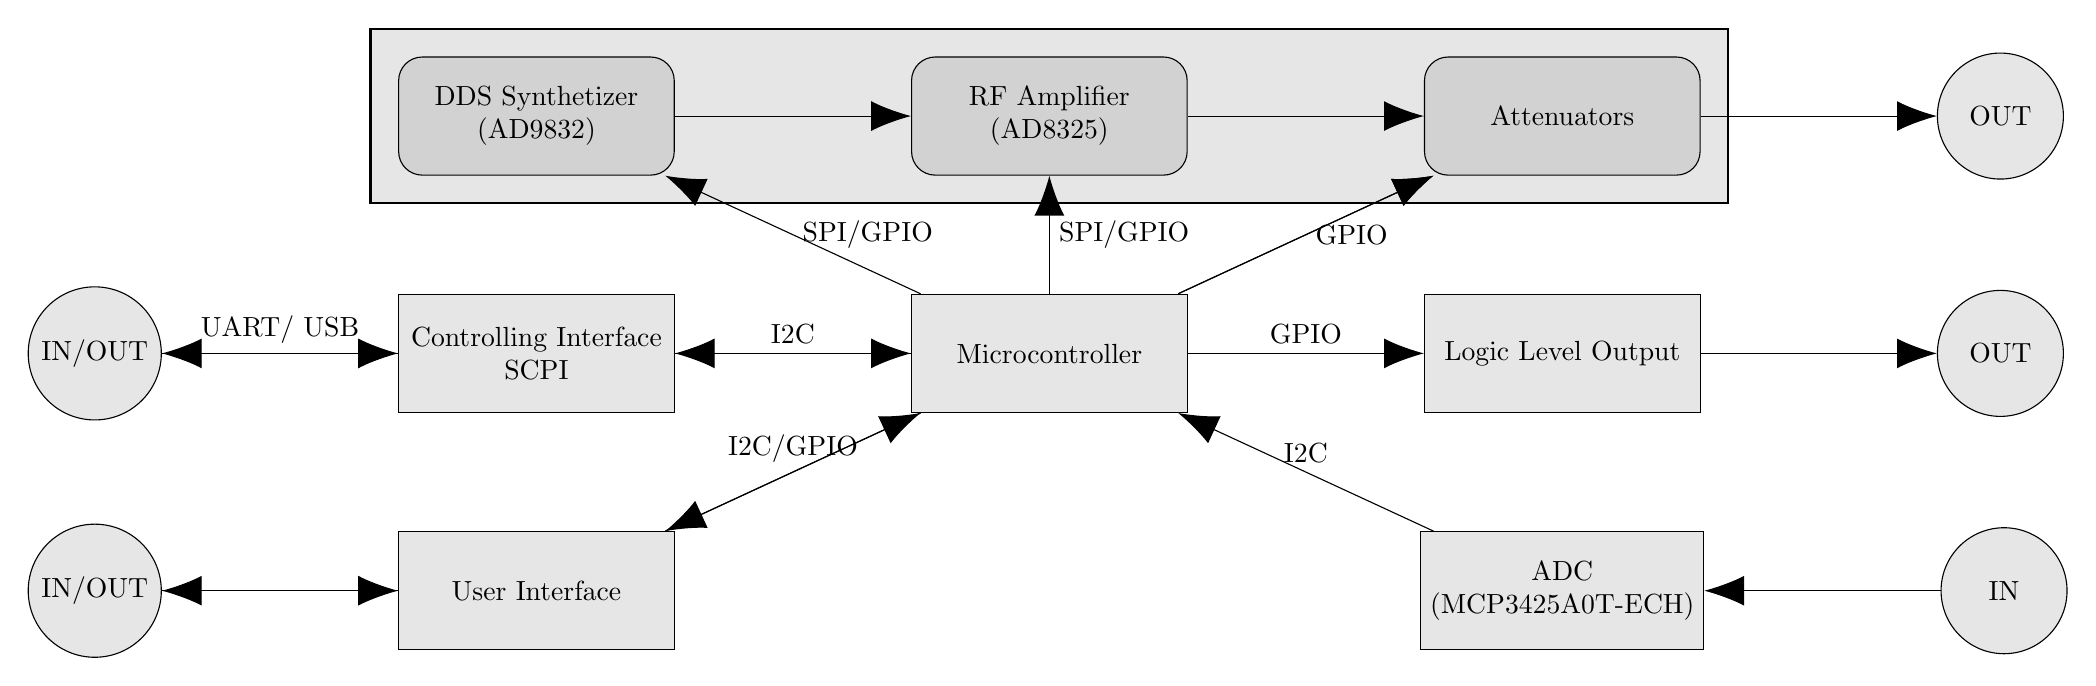
\begin{tikzpicture}[node distance=1.5cm and 3cm]
% Nodes
\pgfdeclarelayer{background}) 
\pgfsetlayers{background,main}

\node (DDSSynthetizer) [component] {DDS Synthetizer\\ (AD9832)};
\node (RFAmplifier) [component, right=of DDSSynthetizer] {RF Amplifier\\ (AD8325)};
\node (Attenuators) [component, right=of RFAmplifier] {Attenuators};


\node (Microcontroller) [system, below=of RFAmplifier] {Microcontroller};
\node (ControllingInterface) [system, left=of Microcontroller] {Controlling Interface\\SCPI};
\node (UserInterface) [system, below=of ControllingInterface] {User Interface};
cage clamp
\node (LogicLevelOutput) [system, below=of Attenuators] {Logic Level Output};
\node (ADC) [system, below=of LogicLevelOutput] {ADC\\ (MCP3425A0T-ECH)};

\node (Output50Ohm) [circle, interface, right=of Attenuators] {OUT};
\node (OutputLogicLevelOutput) [circle, interface, right=of LogicLevelOutput] {OUT};
\node (OutputADC) [circle, interface, right=of ADC] {IN};
\node (OutputControllingInterface) [circle, interface, left=of ControllingInterface] {IN/OUT};
\node (OutputUserInterface) [circle, interface, left=of UserInterface] {IN/OUT};

\begin{pgfonlayer}{background}
\node[system, draw, thick, inner xsep=1em, inner ysep=1em, fit= (DDSSynthetizer) (RFAmplifier) (Attenuators) ] {};
\end{pgfonlayer}

% Connectors
\begin{scope}[->]

\draw [-{Latex[scale=3.0]}] (DDSSynthetizer) -- node[anchor=west, minimum width=.25cm, draw=none] {} (RFAmplifier);
\draw [-{Latex[scale=3.0]}] (RFAmplifier) -- node[anchor=west, minimum width=.25cm, draw=none] {} (Attenuators);

\draw [-{Latex[scale=3.0]}] (Microcontroller) -- node[anchor=west, minimum width=.25cm, draw=none] {SPI/GPIO} (DDSSynthetizer);
\draw [-{Latex[scale=3.0]}] (Microcontroller) -- node[anchor=west, minimum width=.25cm, draw=none] {SPI/GPIO} (RFAmplifier);
\draw [-{Latex[scale=3.0]}] (Microcontroller) -- node[anchor=west, minimum width=.25cm, draw=none] {GPIO} (Attenuators);

\draw [-{Latex[scale=3.0]}] (Microcontroller) -- node[anchor=south, minimum width=.25cm, draw=none] {GPIO} (LogicLevelOutput);
\draw [-{Latex[scale=3.0]}] (Microcontroller) -- node[anchor=west, minimum width=.25cm, draw=none] {} (Attenuators);
\draw [-{Latex[scale=3.0]}] (ADC) -- node[anchor=south, minimum width=.25cm, draw=none] {I2C} (Microcontroller);

\draw [-{Latex[scale=3.0]}] (Microcontroller) -- node[anchor=south, minimum width=.25cm, draw=none] {I2C/GPIO} (UserInterface);
\draw [-{Latex[scale=3.0]}] (UserInterface) -- node[anchor=west, minimum width=.25cm, draw=none] {} (Microcontroller);

\draw [-{Latex[scale=3.0]}] (Microcontroller) -- node[anchor=south, minimum width=.25cm, draw=none] {I2C} (ControllingInterface);
\draw [-{Latex[scale=3.0]}] (ControllingInterface) -- node[anchor=west, minimum width=.25cm, draw=none] {} (Microcontroller);
\end{scope}

\draw [-{Latex[scale=3.0]}] (Attenuators) -- node[anchor=west, minimum width=.25cm, draw=none] {} (Output50Ohm);
\draw [-{Latex[scale=3.0]}] (LogicLevelOutput) -- node[anchor=west, minimum width=.25cm, draw=none] {} (OutputLogicLevelOutput);
\draw [-{Latex[scale=3.0]}] (OutputADC) -- node[anchor=west, minimum width=.25cm, draw=none] {} (ADC);


\draw [-{Latex[scale=3.0]}] (OutputControllingInterface) -- node[anchor=south, minimum width=.25cm, draw=none] {UART/ USB} (ControllingInterface);
\draw [-{Latex[scale=3.0]}] (ControllingInterface) -- node[anchor=west, minimum width=.25cm, draw=none] {} (OutputControllingInterface);

\draw [-{Latex[scale=3.0]}] (OutputUserInterface) -- node[anchor=west, minimum width=.25cm, draw=none] {} (UserInterface);
\draw [-{Latex[scale=3.0]}] (UserInterface) -- node[anchor=west, minimum width=.25cm, draw=none] {} (OutputUserInterface);


\end{tikzpicture}
\end{document}
